Vi har valgt at arbejde med et projekt hvor vi søger at forbedre
arbejdsgangen for røntgenrekvisitioner på Hillerød Hospital. Aktuelt fungerer
rekvisition af billeddannende undersøgelser (eks. røntgen(rtg.)billeder og MR
scanninger) via fax. Dvs. at rekvirenten (lægen), der ønsker et rtg. billede, må
sende en fax til røntgenafdelingen for at udbede sig billedet. Det skaber mange
muligheder for fejl og kan være unødigt kompliceret.
\subsection*{Kort beskrivelse af arbejdsgang (Christian, Magnus)}
\addcontentsline{toc}{subsection}{Kort beskrivelse af arbejdsgang}
I processen hvor et røntgenbillede bestilles, visiteres, bookes, udføres
og vurderes, indgår flere arbejdsgange
(se \hyperref[Rigt_billede]{figur \ref*{Rigt_billede}}).
Rekvisitionen består af en Fax (1.), der afsendes til rtg. afdelingen. Faxen
indscannes af en sekretær (2.) i et visitations/bookingsystem (- en arbejdsgang,
som vi gerne vil gøre overflødig). Herefter vurderes rekvisitionen af en
visitator (røntgenlæge), der vurderer om undersøgelsen er berettiget - visiterer
rekvisitionen (3). Herefter er rekvisitionen enten godkendt eller afvist (4.)\\
\indent Undersøgelsen bookes af en sekretær (Ikke vist). Når det planlagte
tidspunkt er nået hentes patienten fra afdelingen og patienten undersøges (5.).
Ud af undersøgelsen kommer et antal billeder, der lagres i et billedsystem (6.).
Billederne gennemses af en røntgenlæge, der skriver en  røntgenbeskrivelse (7.).
Herefter kan rekvirenten se beskrivelsen i systemet (8.).
\FloatBarrier
\begin{figure}[h]
\centering
\makebox[\textwidth]{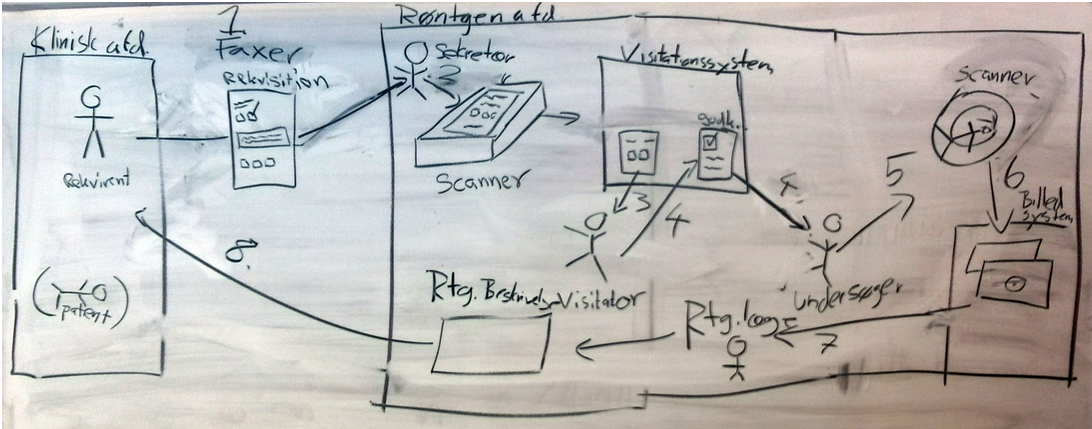
\includegraphics[width=\textwidth]{Rigt_billede}}
\caption{\emph{Rigt billede af arbejdsgangen}: Skitse udarbejdet efter
brugerbeskrivelser.\label{Rigt_billede}}
\end{figure}
\FloatBarrier
\indent Den del af processen vi interesserede os for i første omgang var selve
rekvisitions- og visitationsprocessen. Implementering af bookingsystem, og
billedbeskrivelse var for omfangsrigt til at vi kunne gå i dybden med det.
Integration med udførelsen af undersøgelsen, kræver større kendskab til det
billeddannende udstyr og deres interfaces og er urealistisk at implementere,
vores interessent-interview viste desuden at dette er en del af det nuværende
system, der fungerede godt. Røntgensvaret ligger ligeledes i det eksisterende
system, bundet til billedet, og er således heller ikke realistisk at
implementere i en rekvisitionsløsning.\\
\indent En oplagt udvidelsesmulighed var at implementere muligheden for at
rekvirenten kan se hvor langt i arbejdsgangen rekvisitionen er - om den er
modtaget, visiteret, booket m.m.
\subsection*{Proces og foranalyse (Christian, Martin)}
\addcontentsline{toc}{subsection}{Proces og foranalyse}
Vi valgte at organisere os med en projektleder og 2. leder således at
der på et hvert tidspunkt var én til at sikre at opgaver bliver udført. Desuden
uddelte vi kritiske ansvarsområder til separate medlemmer i gruppen. Vi
udformede en samarbejdskontrakt (se \hyperref[Bilag2]{bilag 2}) for at sikre at
vi havde en måde at afbøde samarbejdsproblemer.\\
\indent Vores største problemer tidligere har været at begrænse omfanget af
vores projekt og at færdiggøre delopgaver/projekt i tide - hvorfor vi har aftalt
særligt fokus på at undgå ‘feature creep’ og bedre kontrol at udviklingsflow. Vi
valgte at implementere en modificeret SCRUM backlog i forsøget på at danne os
overblik over fremdriften i projektet (se \hyperref[Bilag3]{bilag 3}). Vi satte
desuden en deadline for implementeringen- således at sidste iteration kun
drejede sig om test, bugfixing og dokumentation.
\subsubsection*{Værktøjer}
\addcontentsline{toc}{subsubsection}{Værktøjer}
Vi valgte Google Docs, Software Ideas Modeler (SIM) og Github til at håndtere
data og samarbejde, da værktøjerne før har vist sig fleksible og robuste. Vi
brugte Google Docs, da det har den fordel at vi alle kan arbejde samtidig i
dokumenter. Vi brugte SIM til at lave diagrammer, da det understøtter de fleste
af de relevante diagramtyper og vi har erfaring med værktøjet. Vi anvendte
Github, da det har vist sig driftsikkert og integreres godt med eclipse. Vi
valgte at anvende et online tool - audao\cite{audao} - til at generere
basale Data Access Objects (DAO). Det kan, fra en XML beskrivelse af
datamodellen, generere alle de nødvendige DAO og Data Transfer Objects (DTO)
klasser til databasen. CRUD operationer er således autogenererede, men mere
avancerede sql forespørgsler og triggers har vi skrevet selv. Vi valgte at
anvende HeidiSQL som interface til databasen, da vi har gode erfaringer med det.
HeidiSQL\cite{heidisql} er et brugervenligt og overskueligt opensource værktøj
til adninistraion af SQL databaser. Til bruger accept test har vi anvendt
SurveyMonkey\cite{surveymonkey} til oprettelse og hosting af spørgeskema.
\subsubsection*{Kvalitetskriterier (Magnus)}
\addcontentsline{toc}{subsubsection}{Kvalitetskriterier}
Vores kvalitetskriterier er primært at det skal være lettere og hurtigere at at
bestille en undersøgelse. Vi vil opnå begge disse ved at erstatte den nuværende
papirbaserede arbejdsgang med et digitalt system, der kan undgå repeterende
data, håndtere kontrolskemaer, og generelt lette en arbejdstung manuel
fremgangsmåde. Den bedste måde at checke om vi har opnået disse vil nok være via
et spørgeskema udleveret til brugerne, dog er det, grundet generel travlhed i
det danske sygehussystem, usikkert om vi kan få respons på dette.
\subsection*{Risikoanalyse (Rúni, Magnus)}
\addcontentsline{toc}{subsection}{Risikoanalyse}
Initielt udførte vi en risikoanalyse for at identificere de umiddelbare ricisi i
projektet, som vi skulle adressere.\\
\FloatBarrier
\begin{figure}
\begin{tabularx}{\textwidth}{| X | l | l | X | l | l |}
\hline
Risiko & Sandsynlighed & Impact & RMMM & Prioritet & RE\\ \hline
Manglende adgang til enkelte interessenter & 75\% & 5 & Afklar hurtigt hvilke
interessenter og hvad vi gør for erstatning & medium & 3,75\\
\hline

Dårlig time-estimering & 75\% & 5 & Tidsplanlægning opdateres løbende, og
eventuelt uopnåelige mål flyttes til næste iteration eller skæres fra. & medium
& 3,75\\ 
\hline \hline

Opgaven bliver for stor & 25\% & 9 & Starte med den centrale usecase og udvikle
den færdig, således at vi efter hver iteration har et færdigt produkt der kan
afleveres. & høj & 2,25\\
\hline

Begrænset adgang pga. sensitive patient data & 90\% & 2 & Begrænset betydning -
projektet kan gennemføres uden 'real life' data. & lav & 1,8\\
\hline

Manglende adgang til dokumenter & 10\% & 8 & Afklar hurtigt adgang til
dokumenter & høj & 0,8\\
\hline

Manglende erfaring / implementerings vanskeligheder & 10\% & 2 & Eventuelle
implementerings problemer løses fælles, eller kan i værste fald skæres fra. &
lav & 0,2\\
\hline
\end{tabularx}
\caption{\emph{Risiko tabel}: sorteret efter Risk Exposure.\label{risiko_tabel}}
\end{figure}
\FloatBarrier
\indent For at undgå problemet med manglende adgang til interessenter sørgede vi
allerede tidligt i vores forløb for at kontakte Hillerød hospitals
røntgenafdeling og fik en aftale i stand. Problemer med tidsplanlægningen
forsøgte vi at afbøde ved at planlægge opgaver i god tid, og bruge
tidsplanlægningsværktøjer så som en backlog og et PERT diagram. Vi prioriterede
vores mål og kunne skære de mindre væsentlige fra, da projektet kom i tidsnød.
\subsection*{Planlægning (Christian)}
\addcontentsline{toc}{subsection}{Planlægning}
Vi skabte overblik over vores projekt ved at opstille et antal veldefinerede
opgaver for den nærmeste fremtid og konstruerede et basalt PERT diagram
(se \hyperref[Bilag4]{bilag 4}) for at opklare bindinger og estimere et
tidsforbrug. Vi søgte at opdele projektet i mindre 'bidder', således at vi
arbejdede i 3 'sprints'/iterationer. Vi valgte at sætte afleveringen af vores
første prototype, udviklet som mockup i Google Forms og Excel, som første
milestone. Herefter arbejdede vi videre med kravspecifikation, analyse og design
ud fra de inputs brugerne gav os. Desuden lagde vi os fast på og startede på en
implementering i Java/jsp og MySQL. Anden milestone blev afleveringen af vores
fungerende online prototype til fornyet brugertest, hvorefter tredje iteration
blev sat af til rapportfærdiggørelse, intensivering af tests og bugfixing.